\clearpage\section{Bus}
Buses supply seven reference conditions. Empirical transfer reproduces the observed stop fraction more closely in this class, yet its travel-distance discrepancy is larger. A closer match in the total time spent nearly stationary does not specify where those stationary intervals occur or how far the vehicle travels between them.

The fixed request contains eight candidates. The random, image and coordinate rules returned candidate indices 4, 4 and 7, respectively. The observed class stop fraction across the 7 references is 29.5\%.

\begin{center}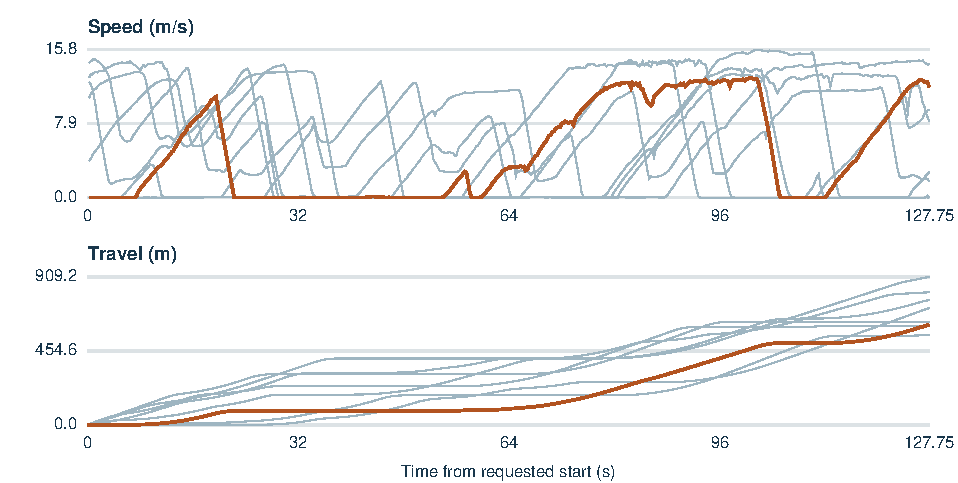
\includegraphics[width=.98\linewidth]{figures/case-bus.pdf}\end{center}
\noindent The highlighted line is the GAF-selected trace. The seven other trajectories are shown in blue-gray. Axes are scaled separately for each class.
\tab{All-candidate bus results. Units are m/s, m/s$^2$, m and percent, respectively.}{case1}{\begin{tabular}{lrrrr}\toprule
Motion & Speed $\W$ & Accel. $\W$ & Travel $\W$ & Stop \%\\\midrule
Diffusion & 0.736 & 0.078 & 95.242 & 22.3\\
Empirical & 0.985 & 0.108 & 180.760 & 31.4\\\bottomrule\end{tabular}}
\FloatBarrier

\clearpage\section{Motorcycle}
The four motorcycle references spend roughly a quarter of sampled intervals below the stop threshold. Both generators spend only about seven percent. Transporting observed profiles from the training library therefore leaves a substantial mismatch even before a learned motion distribution is used. Whether the gap reflects different route mixes or insufficient training coverage requires independent conditions.

The fixed request contains eight candidates. The random, image and coordinate rules returned candidate indices 119, 116 and 115, respectively. The observed class stop fraction across the 4 references is 24.6\%.

\begin{center}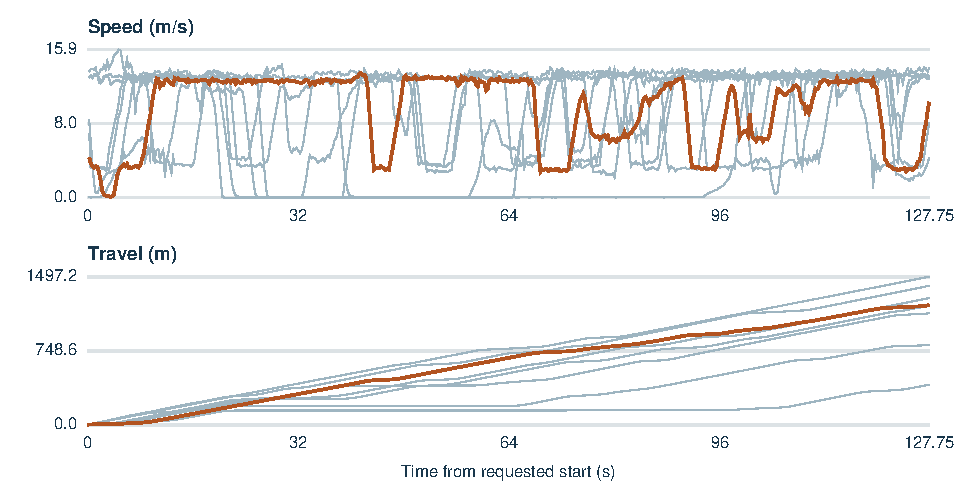
\includegraphics[width=.98\linewidth]{figures/case-motorcycle.pdf}\end{center}
\noindent The highlighted line is the GAF-selected trace. The seven other trajectories are shown in blue-gray. Axes are scaled separately for each class.
\tab{All-candidate motorcycle results. Units are m/s, m/s$^2$, m and percent, respectively.}{case2}{\begin{tabular}{lrrrr}\toprule
Motion & Speed $\W$ & Accel. $\W$ & Travel $\W$ & Stop \%\\\midrule
Diffusion & 2.068 & 0.199 & 347.655 & 7.0\\
Empirical & 2.758 & 0.265 & 367.777 & 7.4\\\bottomrule\end{tabular}}
\FloatBarrier

\clearpage\section{Private car}
Private cars account for 33 of the 53 requests. Their stop fraction is closely matched by diffusion, and their travel discrepancy is smaller than with empirical transfer. The empirical baseline, however, gives a much smaller acceleration discrepancy for this class. These results distinguish agreement on total distance from agreement on changes in speed.

The fixed request contains eight candidates. The random, image and coordinate rules returned candidate indices 133, 133 and 135, respectively. The observed class stop fraction across the 33 references is 4.8\%.

\begin{center}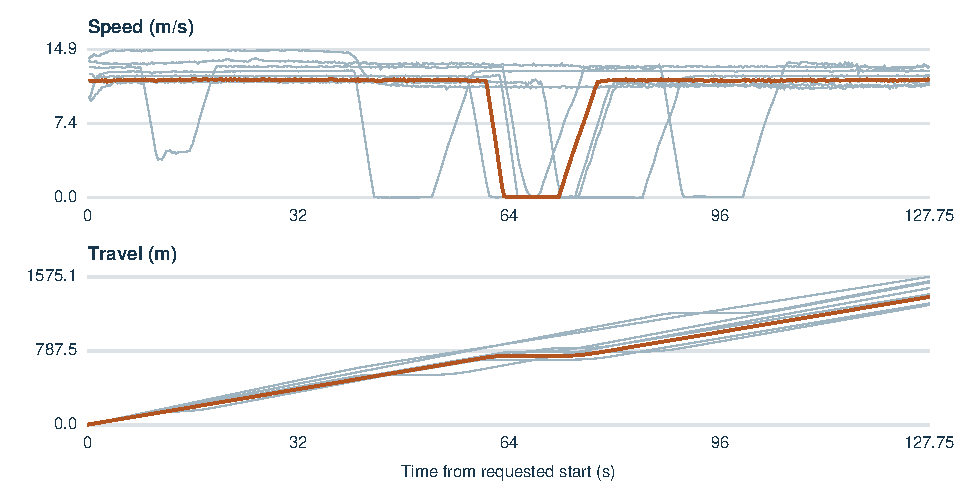
\includegraphics[width=.98\linewidth]{figures/case-private_car.pdf}\end{center}
\noindent The highlighted line is the GAF-selected trace. The seven other trajectories are shown in blue-gray. Axes are scaled separately for each class.
\tab{All-candidate private car results. Units are m/s, m/s$^2$, m and percent, respectively.}{case3}{\begin{tabular}{lrrrr}\toprule
Motion & Speed $\W$ & Accel. $\W$ & Travel $\W$ & Stop \%\\\midrule
Diffusion & 0.356 & 0.187 & 51.620 & 4.8\\
Empirical & 0.985 & 0.058 & 124.766 & 3.8\\\bottomrule\end{tabular}}
\FloatBarrier

\clearpage\section{Bicycle}
The seven observed bicycle windows spend little sampled time below the stop threshold. The two generators produce similar stop fractions of about three percent. Both acceleration discrepancies are comparatively large. Since acceleration here differentiates planar speed, quarter-second variations in the decoded geometry and timing can affect this metric even on a connected route.

The fixed request contains eight candidates. The random, image and coordinate rules returned candidate indices 62, 59 and 61, respectively. The observed class stop fraction across the 7 references is 0.1\%.

\begin{center}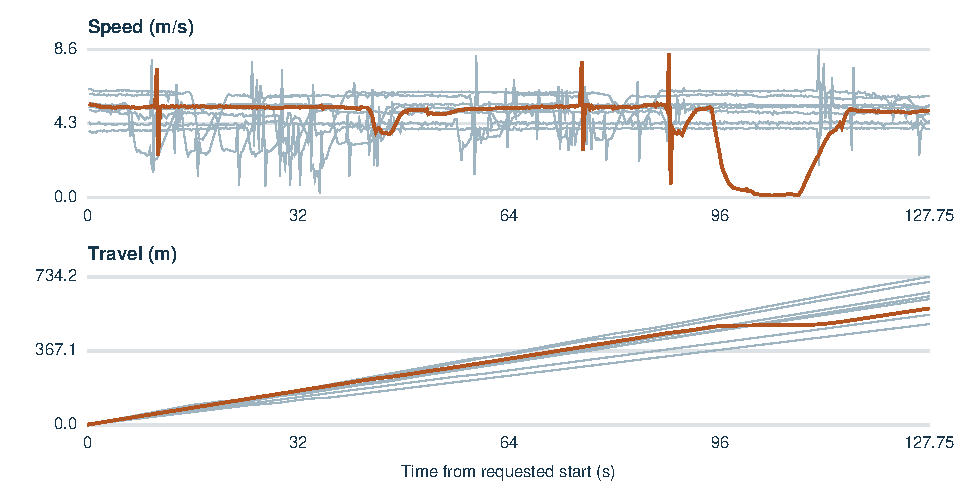
\includegraphics[width=.98\linewidth]{figures/case-bycicle.pdf}\end{center}
\noindent The highlighted line is the GAF-selected trace. The seven other trajectories are shown in blue-gray. Axes are scaled separately for each class.
\tab{All-candidate bicycle results. Units are m/s, m/s$^2$, m and percent, respectively.}{case4}{\begin{tabular}{lrrrr}\toprule
Motion & Speed $\W$ & Accel. $\W$ & Travel $\W$ & Stop \%\\\midrule
Diffusion & 0.378 & 0.651 & 55.534 & 3.0\\
Empirical & 0.505 & 0.607 & 74.275 & 3.0\\\bottomrule\end{tabular}}
\FloatBarrier

\clearpage\section{Taxi or Uber}
Only two taxi requests supply the reference distribution. In this class empirical transfer has smaller speed and travel discrepancies than diffusion, while both generators spend considerably less time nearly stationary than the two observed vehicles. The direction of the class-specific result is informative, but two vehicles provide very little information about the broader taxi population.

The fixed request contains eight candidates. The random, image and coordinate rules returned candidate indices 247, 241 and 247, respectively. The observed class stop fraction across the 2 references is 19.2\%.

\begin{center}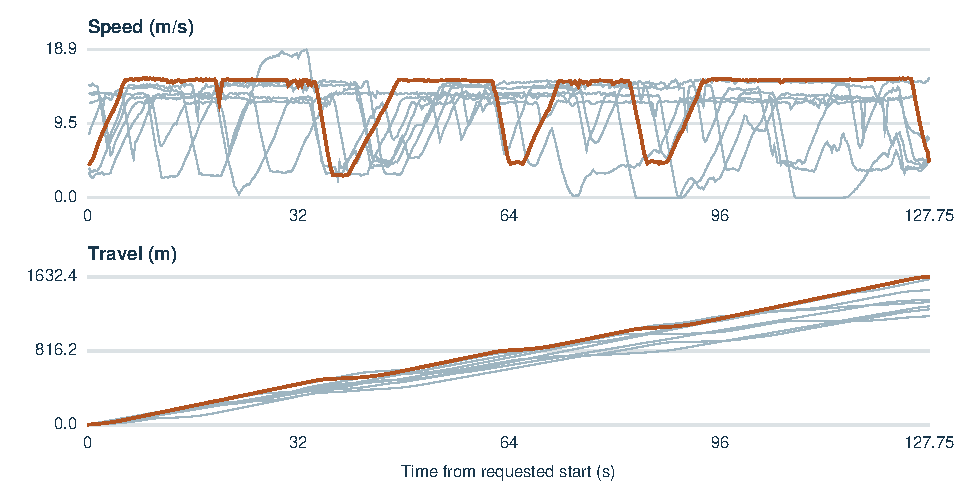
\includegraphics[width=.98\linewidth]{figures/case-taxi_or_uber.pdf}\end{center}
\noindent The highlighted line is the GAF-selected trace. The seven other trajectories are shown in blue-gray. Axes are scaled separately for each class.
\tab{All-candidate taxi or uber results. Units are m/s, m/s$^2$, m and percent, respectively.}{case5}{\begin{tabular}{lrrrr}\toprule
Motion & Speed $\W$ & Accel. $\W$ & Travel $\W$ & Stop \%\\\midrule
Diffusion & 2.681 & 0.231 & 337.019 & 2.2\\
Empirical & 2.000 & 0.155 & 258.019 & 5.3\\\bottomrule\end{tabular}}
\FloatBarrier
